\documentclass[11pt]{article}
\usepackage[utf8]{inputenc}
\usepackage{circuitikz}
\usepackage{longtable}
\usepackage{multicol}
\usepackage{stmaryrd}
\usepackage{titlesec}
\usepackage{graphicx}
\usepackage{amsmath}
\usepackage{amssymb}
\usepackage{float}
\usepackage{color}
\usepackage{pbox}
\usepackage[txtcentered=true, height=40pt, width=70pt]{thumbs}
\usepackage[left=2.5cm, top=2.5cm, right=3cm]{geometry}
\usepackage[justification=centering]{caption}
\usepackage{geometry}
\DeclareGraphicsExtensions{.png}

\newcommand{\fancythumb}[2]{
	\addthumb{#1}{\large\sffamily\textbf{\space\space#1\vspace{5pt}}}{white}{#2}
}

\newcommand{\fancyformula}[2]{
	\small
	\raggedright\sffamily\textbf{#1}
	#2
}

% Subsections with letters (for appendix)
\renewcommand{\thesubsection}{\Alph{subsection}}

\pagenumbering{arabic}
\titleformat*{\section}{\sffamily\huge\bfseries}
\titleformat*{\subsection}{\sffamily\Large\bfseries}
\titleformat*{\subsubsection}{\sffamily\large\bfseries}
\setlength{\multicolsep}{4.0pt}

\begin{document}
\section*{Gleichstrommaschine}
\fancythumb{GSM}{teal}

\subsection*{Einphasiges Ersatzschaltbild}
\begin{figure}[h]\centering
	\begin{circuitikz}[european, scale=1, font=\large]
	\draw
		(0,3)
		to [R=$R_V$, n=Rv, o-](3,3)
		to [short, i=$I~\textnormal{=}~I_a$, o-](4,3)
		to [R=$R_a$](6,3)
		to [short](7,3)
		to [V=$U_i$](7,0)
		to [short, -o](3,0)
		to [short, -o](0,0)
		(10,3)
		to [short, o-](13,3)
		to [R=$R_e$](13,0) 
		to [short, -o](10,0)
		(Rv.s) node[below] {\tiny(optional)};

	\draw[->, >=latex] (0,2.8) -- (0,0.2) node [pos=0.5, left] {$U$};
	\draw[->, >=latex] (3,2.8) -- (3,0.2) node [pos=0.5, left] {$U_a$};
	\draw[->, >=latex] (10,2.8) -- (10,0.2) node [pos=0.5, left] {$U_e$};
	\end{circuitikz}
	\caption*{Ersatzschaltbild des Ankers (Rotor, links) und des Erregers (Stator, rechts)}
\end{figure}

\subsection*{Leistungsbilanz}
\begin{figure}[h]
	\centering
	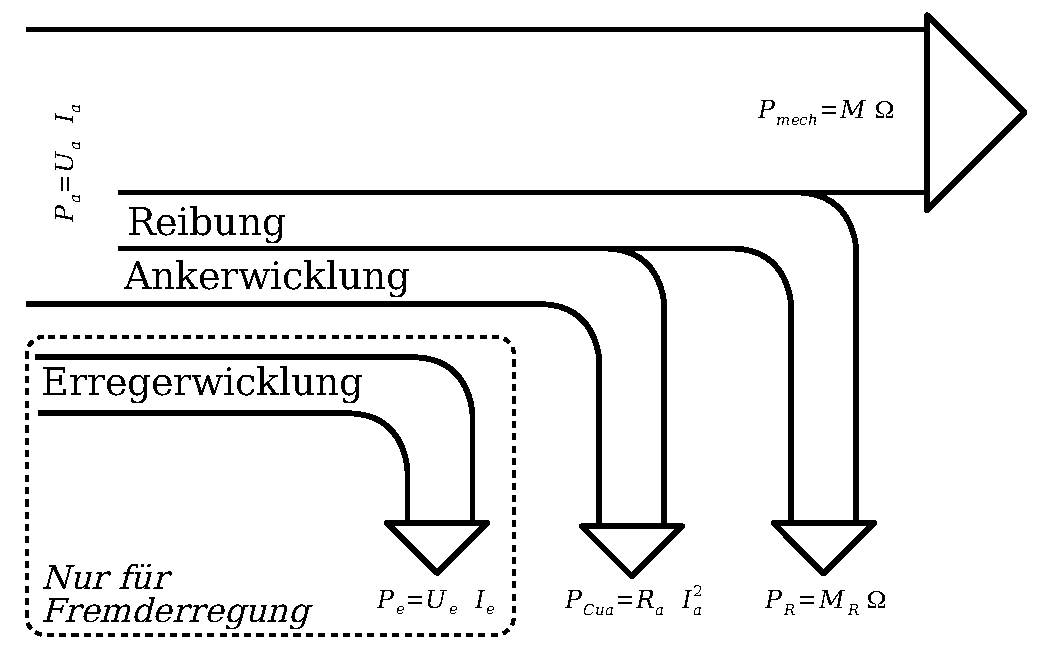
\includegraphics[width=0.7\textwidth]{img/gleichstrommaschine_leistungsbilanz.pdf}
	\caption*{Hier gilt die Annahme $R_V = 0$, d.h. kein Vorschaltwiderstand}
\end{figure}

\subsection*{Kenngrößen}
\textbf{Es gelte hier überall $R_V = 0$!}

\begin{center}
\bgroup
\begin{longtable}{r p{12cm}}
	\textbf{Stillstand ($\Omega = 0$)} & Im Anker wird keine Spannung induziert, $U_i = 0$. Die Maschine bringt das Stillstandsdrehmoment $M_{st} = K ~ \Phi ~ \frac{U}{R_a} = K ~ \Phi ~ I_{st}$ auf. Im Ankerkreis fließt $I_{st} = \frac{U}{R_a}$ \\
	\textbf{Leerlauf ($M_i = 0$)} & Es wird keine Leistung umgesetzt, d.h. $I = 0$. Folglich ist $U_i = U$. Für die Drehzahl folgt $\Omega_\ell = \frac{U}{K ~ \Phi}$. \\
	\textbf{Nennwerte} & Es werden die maximalen Bemessungswerte $U_N$, $I_N$, $I_{eN}$ angegeben, die nicht längerfristig überschritten werden dürfen. \\
	\textbf{Motorbereich} & GSM dreht sich langsamer als $n_{\ell N}$ vorwärts, d.h. $0 \leq s \leq 1$, $P_{mech} \approx P_{el} > 0$. \\
	\textbf{Generatorbereich} & GSM dreht sich schneller als $n_{\ell N}$ vorwärts, d.h. $s < 0$, $P_{mech} \approx P_{el} < 0$. \\
	\pbox{20cm}{\textbf{Gegenstrom-} \\ \textbf{bremsbereich}} & GSM dreht sich rückwärts, d.h. $s > 1$, $P_{mech} < 0$ und $P_{el} > 0$.
\end{longtable}
\egroup
\end{center}

\subsection*{Momentenkennlinie}

\subsection*{Formeln}
\textbf{Es gelte hier überall $R_V = 0$!}

\begin{multicols}{2}
\fancyformula{Grundgleichung: Induzierte Spannung}{
	\[
		U_i = K ~ \Phi ~ \Omega
	\]
}

\fancyformula{Grundgleichung: Inneres Drehmoment}{
	\[
		M_i = K ~ \Phi ~ I
	\]
}

\fancyformula{Grundgleichung: Maschengleichung}{
	\[
		I = \frac{U - U_i}{R_a}
	\]
}

\fancyformula{Grundgleichung: Erregerfeld-Hauptfluss}{
	(nur bei Fremderregung)
	\[
		\Phi = c_1 ~ I_e
	\]
}

\fancyformula{Schlupf}{
	\[
		s = 1 - \frac{n}{n_{\ell N}}
	\]
}

\fancyformula{Drehmoment aus Stillstandsdrehmoment}{
	\[
		M_i = s ~ M_{stN}
	\]
}

\fancyformula{Drehmoment aus Nenndrehmoment}{
	\[
		\frac{M_i}{M_{iN}} = \frac{s}{s_N}
	\]
}

\fancyformula{Inneres Drehmoment}{
	\[
		M_i = \frac{K ~ \Phi}{R_a} ~ (U - K ~ \Phi ~ \Omega)
	\]
}

\end{multicols}

\raggedright
\vspace{12pt}
\footnotesize
\begin{tabular}{r p{13cm}}
	\sffamily\textbf{Indizes:} & \rmfamily \textbf{i} = Inneres Drehmoment, \textbf{$\ell$} = Leerlauf, \textbf{N} = Spannung hat Nennwert, \textbf{a} = Anker (Rotor), \textbf{e} = Erreger (Stator), \textbf{st} = Stillstand
\end{tabular}
\normalsize


\newpage
\section*{Asynchronmaschine}
\fancythumb{ASM}{red}
\subsection*{Einphasiges Ersatzschaltbild}
\begin{figure}[h]\centering
	\begin{circuitikz}[european, scale=1, font=\large]
	\draw
		(0,3)
		to [short, i=$\underline{I}_1$, o-](1.0,3)
		to [L=$L_{\sigma1}$](3,3)
		to [short](4.0,3)
		to [L=$L_{h1}$, i>_=$\underline{I}_{m1}$, *-*] (4,0)
		(4.0,3.0)
		to [L=$L_{\sigma2}'$](7.0,3.0)
		to [R=$R_{2}' ~ \frac{1}{s}$, i>^=$\underline{I}_1^i$](10.0,3)
		to [R, l_=$R_{2Z}' ~ \frac{1}{s}$] (10.0,0) 
		to [short, -o]	(0,0);

	\draw[->, >=latex] (0,2.8) -- (0,0.2) node [pos=0.5, left] {$\underline U_1$};
	\end{circuitikz}
	\caption*{Man beachte die schlupfabhängigen Widerstände}
\end{figure}

\subsection*{Leistungsbilanz}
\begin{figure}[h]
	\centering
	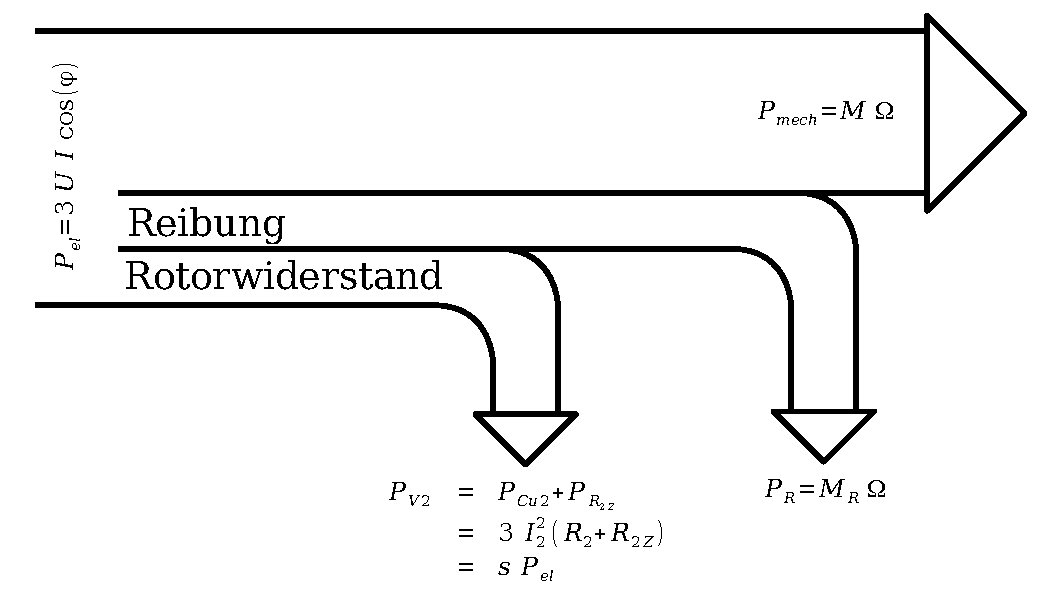
\includegraphics[width=0.7\textwidth]{img/asynchronmaschine_leistungsbilanz.pdf}
	\caption*{Sonstige Verluste vernachlässigt, mit $I_2$…Läuferstrom, häufig gilt $R_{2Z} = 0$}
\end{figure}

\subsection*{Kenngrößen}
\begin{center}
\bgroup
\begin{longtable}{r p{12cm}}
	\textbf{Kippunkt} & Arbeitspunkt des maximalen Drehmoments (\textit{Kippmoment $M_{iK}$}), welches die Maschine abgeben kann (bzw. im Generatorbetrieb aufnehmen kann). Es tritt der \textit{Kippschlupf} $s_K$ auf, wobei ein Zusammenhang über die Kloss'sche Formel gegeben ist. \\
	\textbf{Leerlaufpunkt} & Arbeitspunkt, an dem keine elektrische / mechanische Leistung umgesetzt wird. Es gilt $s = 0$ für den Schlupf und $M_i = 0$ für das Drehmoment, die Maschine dreht sich mit ihrer \textit{Leerlaufdrehzahl} $n_0 = \frac{\Omega_0}{2\pi}$. \\
	\textbf{Nennpunkt} & Arbiträr festgelegter, vorgesehener Betriebspunkt. Häufig dürfen Statorstrom und -spannung diese Nennwerte nicht überschreiten. Typischerweise $s = 2\dots4\%$. \\
	\textbf{Anlaufpunkt} & Punkt, an dem die ASM stillsteht, d.h. $s = 1$. Das \textit{Anlaufdrehmoment} berechnet sich mit der Kloss'schen Formel. \\
	\textbf{Motorbereich} & ASM dreht sich langsamer als $n_0$ vorwärts, d.h. $0 \leq s \leq 1$, $P_{mech} \approx P_{el} > 0$. \\
	\textbf{Generatorbereich} & ASM dreht sich schneller als $n_0$ vorwärts, d.h. $s < 0$, $P_{mech} \approx P_{el} < 0$. \\
	\pbox{20cm}{\textbf{Gegenstrom-} \\ \textbf{bremsbereich}} & ASM dreht sich rückwärts, d.h. $s > 1$, $P_{mech} < 0$ und $P_{el} > 0$.
\end{longtable}
\egroup
\end{center}

\subsection*{Stromortskurve (Heylandkreis)}
\begin{figure}[H]
	\centering
	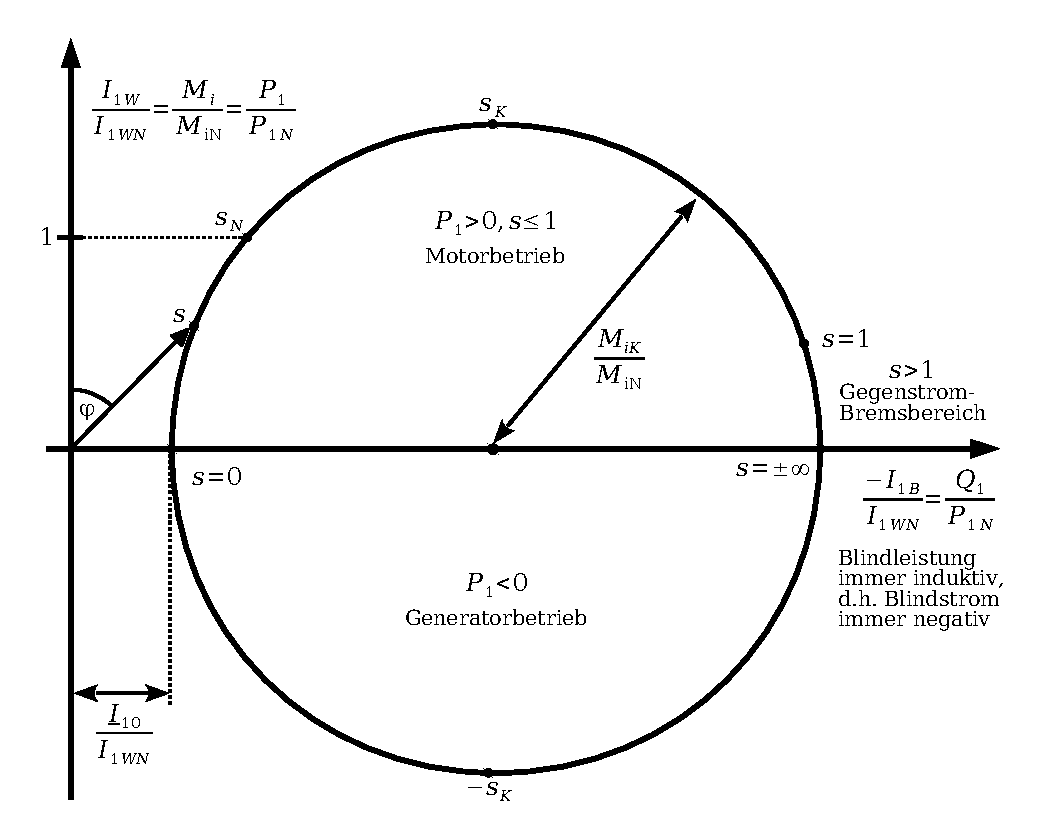
\includegraphics[width=0.9\textwidth]{img/asynchronmaschine_heylandkreis.pdf}
	\caption*{Der Schlupf auf dem Kreisbogen kann entsprechend Anhang \ref{ssec:appendix_asm_slip} abgelesen werden}
\end{figure}

\subsection*{Momentenkennlinie}
\begin{figure}[H]
	\centering
	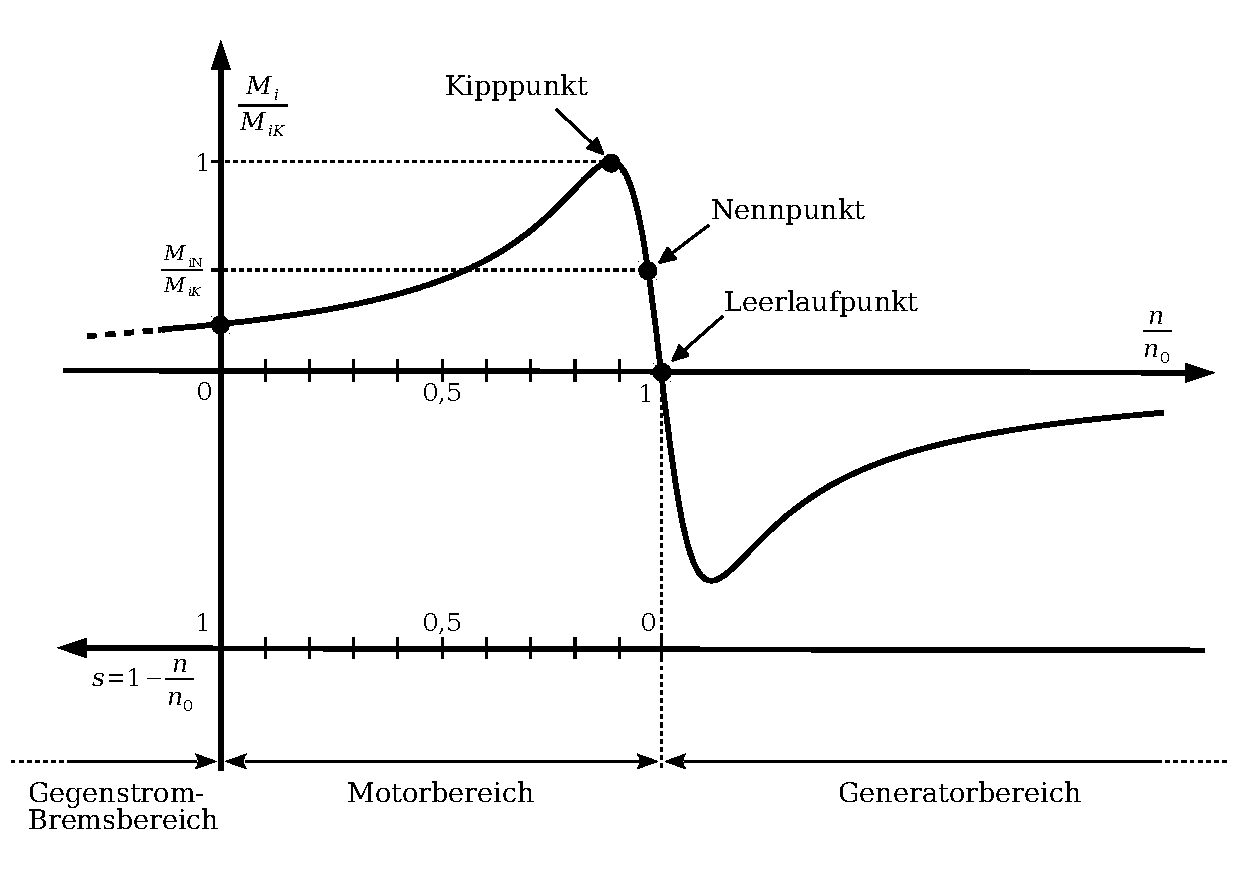
\includegraphics[width=0.9\textwidth]{img/asynchronmaschine_kennlinie.pdf}
	\caption*{Der Verlauf der Kennlinie ist durch die Kloss'sche Formel gegeben}
\end{figure}

\subsection*{Formeln}
\begin{multicols}{2}
\fancyformula{Schlupf}{
	\[
		s = 1 - \frac{n}{n_0}
	\]
}

\fancyformula{Mech. und el. Winkelgeschwindigkeit}{
	\[
		\Omega_0 = \frac{\omega_0}{p}
	\]
}

\fancyformula{Kloss'sche Formel}{
	\[
		\frac{M_i}{M_{iK}} = \frac{2}{\frac{s}{s_K} + \frac{s_K}{s}}
	\]
}

\fancyformula{Kippschlupf ($\Leftrightarrow$ Kloss'sche Formel)}{
	\[
		s_K = s~\left( \frac{M_{iK}}{M_i} \pm \sqrt{\left( \frac{M_{iK}}{M_i} \right)^2 - 1} \right)
	\]
}

\fancyformula{Rotordrehstromfrequenz}{
	\[
		\omega_2 = s ~ \omega_1
	\]
}

\fancyformula{Frequenzumrichterbetrieb bei $\omega_1$ und $U_1$}{
	\[
		\frac{n_0}{n_{0N}} = \frac{\omega_1}{\omega_{1N}} ~~ \mathrm{,} ~~ \frac{s_K}{s_{KN}} = \frac{\omega_{1N}}{\omega_1} ~~ \mathrm{,} ~~ \frac{M_{iK}}{M_{iKN}} = \left(\frac{U_1 ~ \omega_{1N}}{U_{1N} ~ \omega_1}\right)^2
	\]
}

\fancyformula{Proportionalitäten}{
	\[
		\frac{M_i}{M_{iN}} = \frac{I_{1W}}{I_{1WN}} = \frac{P_1}{P_{1N}} \quad \mathrm{und} \quad \frac{-I_{1B}}{I_{1WN}} = \frac{Q_1}{P_{1N}}
	\]
}

\sffamily{\textbf{Verweis:}} \rmfamily Weitere Formeln zu elektrischen Größen und zum Läuferzusatzwiderstand $R_{2Z}$ im Umdruck.
\end{multicols}

\raggedright
\vspace{12pt}
\footnotesize
\begin{tabular}{r p{13cm}}
	\sffamily\textbf{Indizes:} & \rmfamily \textbf{0} = Leerlauf, \textbf{1} = Stator, \textbf{2} = Rotor, \textbf{K} = Kipppunkt, \textbf{N} = Nennbetrieb, \textbf{W} = Wirkstrom, \textbf{B} = Blindstrom, \textbf{i} = inneres Drehmoment
\end{tabular}
\normalsize

\newpage
\section*{Synchronmaschine}
\fancythumb{SM}{magenta}
\subsection*{Ersatzschaltbilder}
\subsubsection*{Vollständiges ESB der Synchronmaschine}
\begin{figure}[h]\centering
	\begin{circuitikz}[european, scale=1, font=\large]
	\draw
		(0,3) to [short, i=$i_1$, o-](1,3)
		to [R=$R_1$](3, 3)
		to [L=$L_{\sigma1}$](5,3)
		to [short, o-](6,3)
		to [L,l_=$L_{h1}$, i>^=$i_{m1}$, *-*] (6,0)
		to [short, -o](5,0)
		to [short, -o](0,0)
		(6,3) to [short, -o](7,3) to [short] (8,3)
		to [sI=$i_1^i$](8,0)
		to [short, -o] (7,0) to [short] (6,0)
		(10,3) to [short, -o, i<_=$I_e$](11,3)
		to [L=$L_{\sigma e}$] (13,3)
		to [R=$R_e$] (15,3)
		to [short, o-] (16,3)
		to [R=$R_{ea}$] (16,1.5)
		to [dcvsource=$u_{ae}$] (16,0)
		to [short, -o] (15,0)
		to [short] (11,0)
		to [short, o-] (10,0)
		to [short] (10,3);
	\draw[->, >=latex] (0,2.8) -- (0,0.2) node [pos=0.5, left] {$u_1$};
	\draw[->, >=latex] (7,2.8) -- (7,0.2) node [pos=0.5, left] {$u_{h1}$};
	\draw[->, >=latex] (11,2.8) -- (11,0.2) node [pos=0.5, right] {$u_{he}=0$};
	\draw[dashed](7,3.5)rectangle(11,-0.5);
	\node at (9,-1) (ideal_SM){ideale SM};
	\draw[dashed](5,4)rectangle(11,-1.5);
	\node at (8,-2) (fest_SM){festgekoppelte SM};
	\end{circuitikz}
\end{figure}

\subsubsection*{Ständerseitiges ESB 1. Art}
\begin{figure}[h]\centering
	\begin{circuitikz}[european, scale=1, font=\large]
	\draw
		(0,3) to [short, i=$i_1$, o-](1,3)
		to [R=$R_1$](3, 3)
		to [L=$L_{\sigma1}$](5,3)
		to [short, o-](6,3)
		to [L=$L_{h1}$, i>^=$i_{m1}$, *-*] (6,0)
		to [short, -o](5,0)
		to [short, -o](0,0)
		(6,3) to [short](8,3)
		to [sI=$i_1^i$](8,0)
		to [short] (6,0);
	\draw[->, >=latex] (0,2.8) -- (0,0.2) node [pos=0.5, left] {$u_1$};
	\end{circuitikz}
	\caption*{$i^i_1=\hat{i}^i_1\cdot cos(\omega t) = \dfrac{2}{3}\cdot\dfrac{w_e\cdot\xi_e}{w_1\cdot\xi_1}\cdot I_e\cdot cos(\omega t)$}
\end{figure}
\newpage
\subsubsection*{Ständerseitiges ESB 2. Art}
\begin{figure}[h]\centering
	\begin{circuitikz}[european, scale=1, font=\large]
	\draw
		(0,3) to [short, i=$i_1$, o-](1,3)
		to [R=$R_1$](3, 3)
		to [L=$L_{\sigma1}$](5,3)
		to [short, o-](6,3)
		to [L=$L_{h1}$, i>^=$\i_{m1}$] (8,3)
		to [sV=$u_p$](8,0)
		to [short] (6,0)
		to [short, -o](5,0)
		to [short, -o](0,0);
	\draw[->, >=latex] (0,2.8) -- (0,0.2) node [pos=0.5, left] {$u_1$};
	\draw[->, >=latex] (5,2.8) -- (5,0.2) node [pos=0.5, left] {$u_{h1}$};
	\end{circuitikz}
	\caption*{$u_p=\omega L_{h1}\cdot\dfrac{2}{3}\cdot\dfrac{w_e\cdot\xi_e}{w_1\cdot\xi_1}\cdot I_e\cdot sin(\omega t)$}
\end{figure}

\subsubsection*{Vereinfachung des ESB 2. Art}
\begin{figure}[h]\centering
	\begin{circuitikz}[european, scale=1, font=\large]
	\draw
		(0,3) to [short, i=$\underline{I}_1$, o-](1,3)
		to [L=$L_{1}$](3,3)
		to [short, -o](4,3)
		(4,0) to [short, o-] (3,0)
		to [short, -o] (0,0);
	\draw[->, >=latex] (0,2.8) -- (0,0.2) node [pos=0.5, left] {$\underline{U}_1$};
	\draw[->, >=latex] (4,2.8) -- (4,0.2) node [pos=0.5, left] {$\underline{U}_p$};
	\end{circuitikz}
	\caption*{$L_1=L_{\sigma1}+L_{h1}$}
\end{figure}

\subsection*{Leistungsbilanz}
\begin{figure}[H]
	\centering
	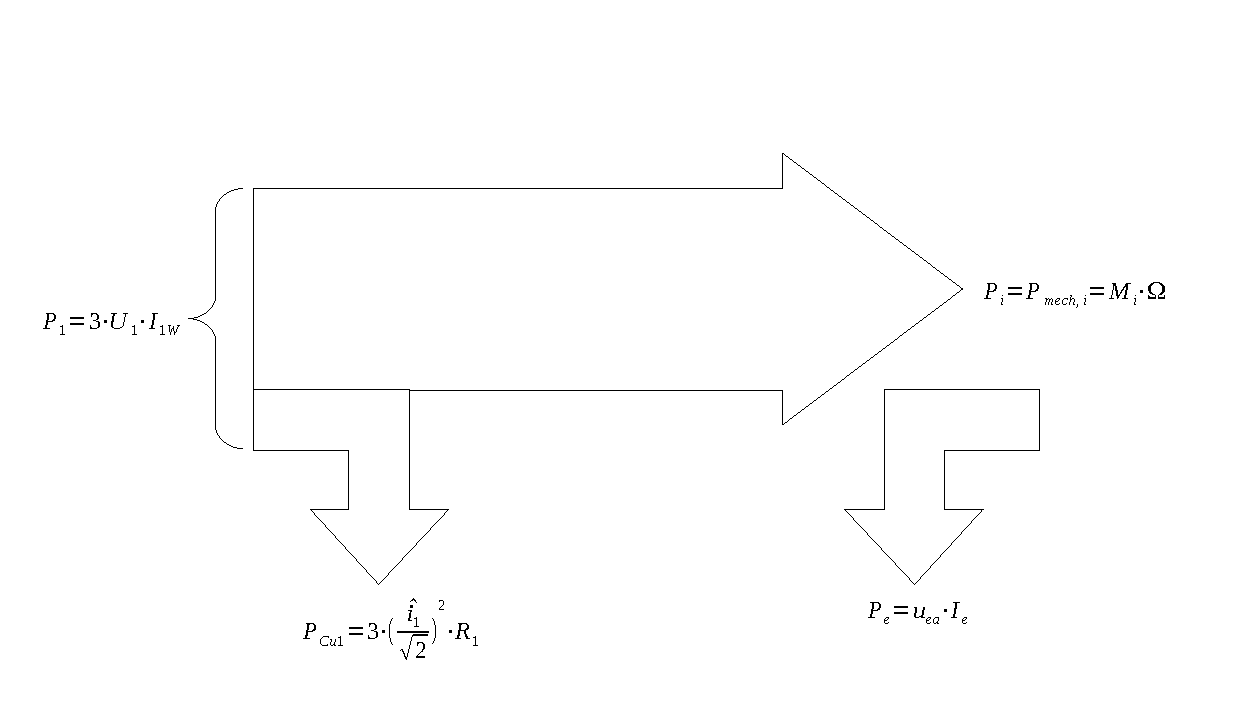
\includegraphics[width=0.5\textwidth]{img/SM_Leistungsbilanz.pdf}
\end{figure}
Die Leistung $P_e$ zur Erregung der Läuferspule geht vollständig verloren.\\
Wenn der Widerstand auf der Ständerseite vernachlässigbar ist ($P_{Cu1} << P_i$), dann gilt die Vereinfachung des ESB 2. Art und $P_i = P_1$. 
\subsection*{Stromortskurve und Kenngrößen}
\begin{figure}[H]
	\centering
	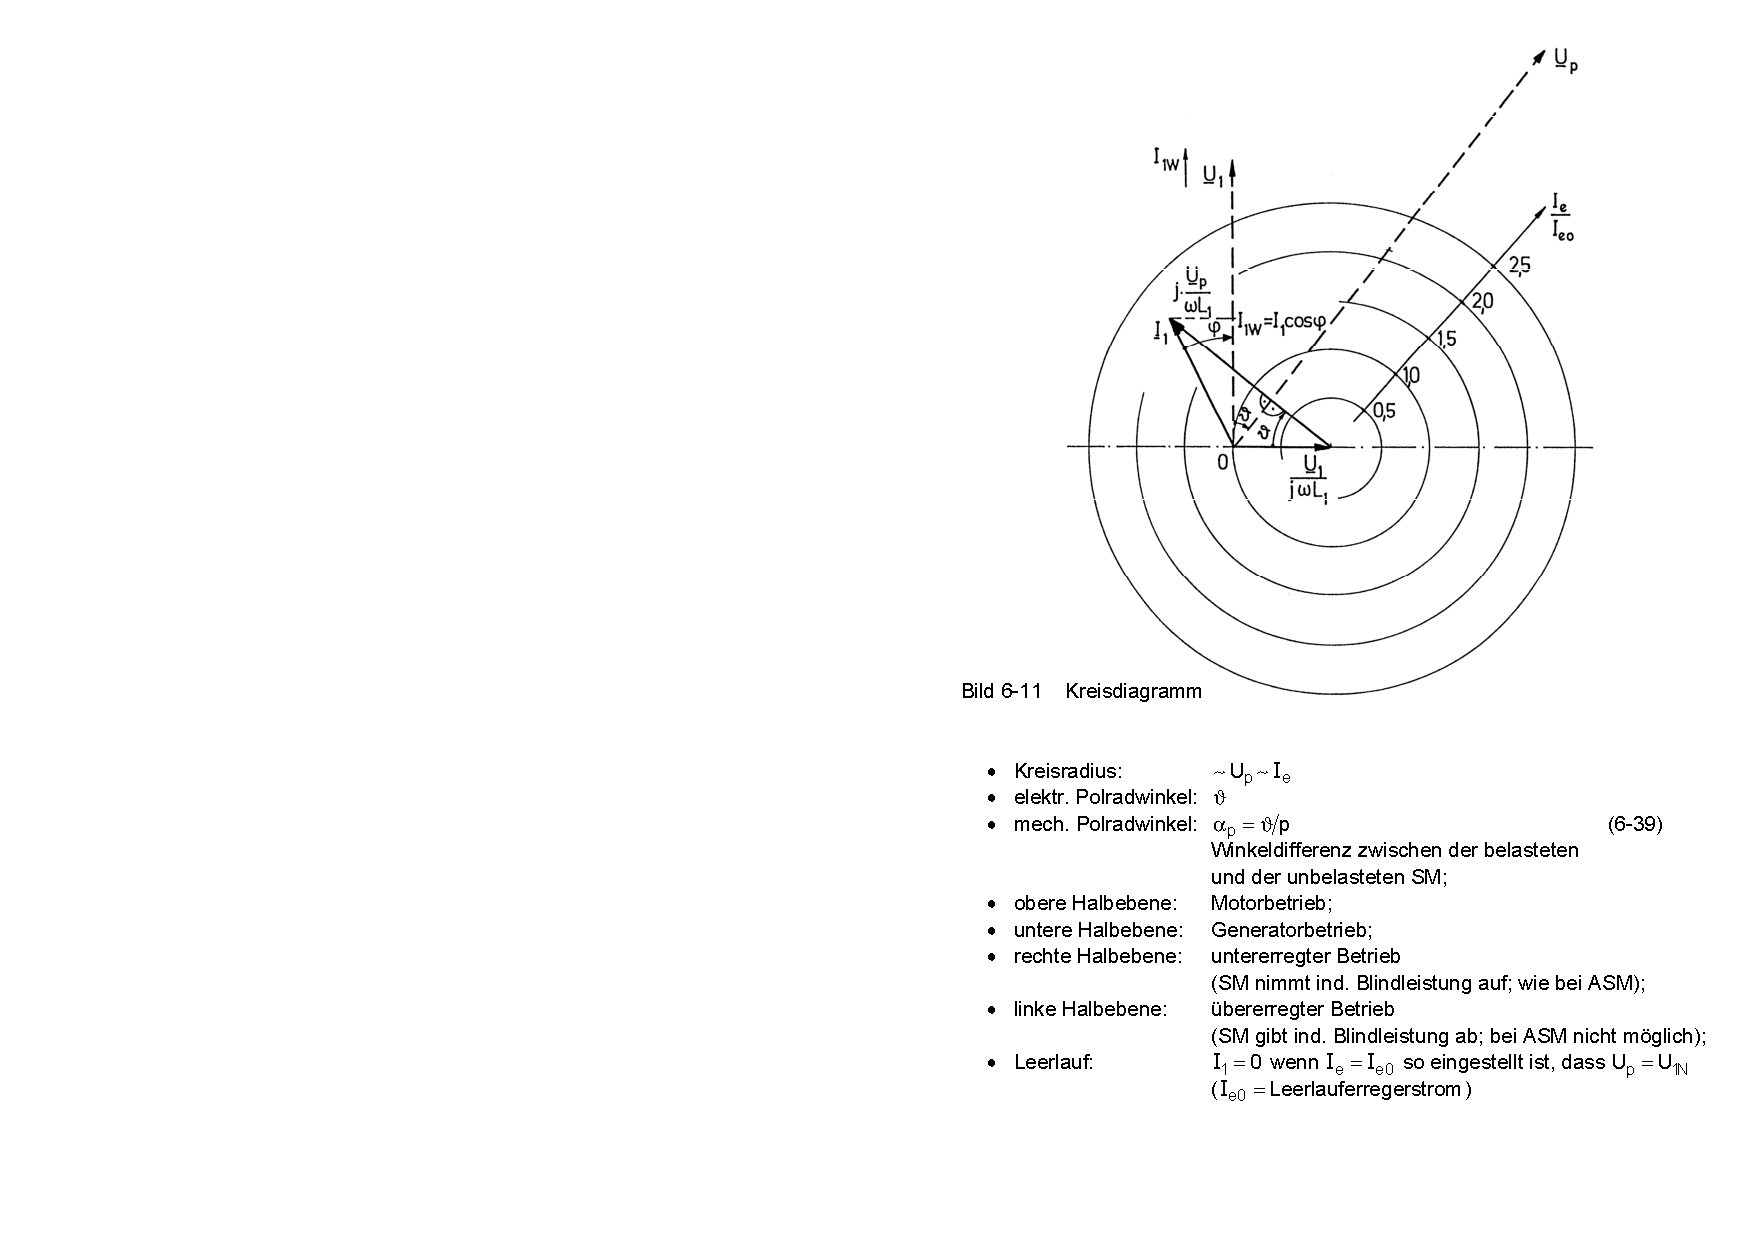
\includegraphics[width=0.7\textwidth]{img/SM_Ortskurve.pdf}
\end{figure}

\textbf{Drehzahl $\Omega$ und $\omega$:}\\
Elektrische Drehzahl $\omega = 2\pi\cdot f_N$, wobei $f_N$ die Netzfrequenz ist. $\rightarrow$ Läuferdrehzahl ist um den Faktor $\dfrac{1}{p}$ kleiner. $\Omega=\dfrac{\omega}{p}$\\

\textbf{Erregerstrom $I_e$:} \\ 
Man spricht vom \textbf{untereregten} Betrieb, wenn die Maschine induktive Blindleistung aufnimmt bzw. kapazitive abgibt $\rightarrow$ Der Stromzeiger $I_1$ zeigt in die rechte Halbebene.\\
Man spricht vom \textbf{übereregten} Betrieb, wenn die Maschine induktive Blindleistung abgibt bzw. kapazitive aufnimmt $\rightarrow$ Der Stromzeiger $I_1$ zeigt in die linke Halbebene.\\

\subsection*{Momentenkennlinie}
Die Synchornmaschine weißt bei jedem abgegebenen oder abverlangten Moment unterhalb des Polradwinkels $\dfrac{\pi}{2}$ die gleiche Drehzahl $\Omega$ auf. Es verändert sich lediglich der Polradwinkel $\theta$.

\begin{figure}[H]
	\centering
	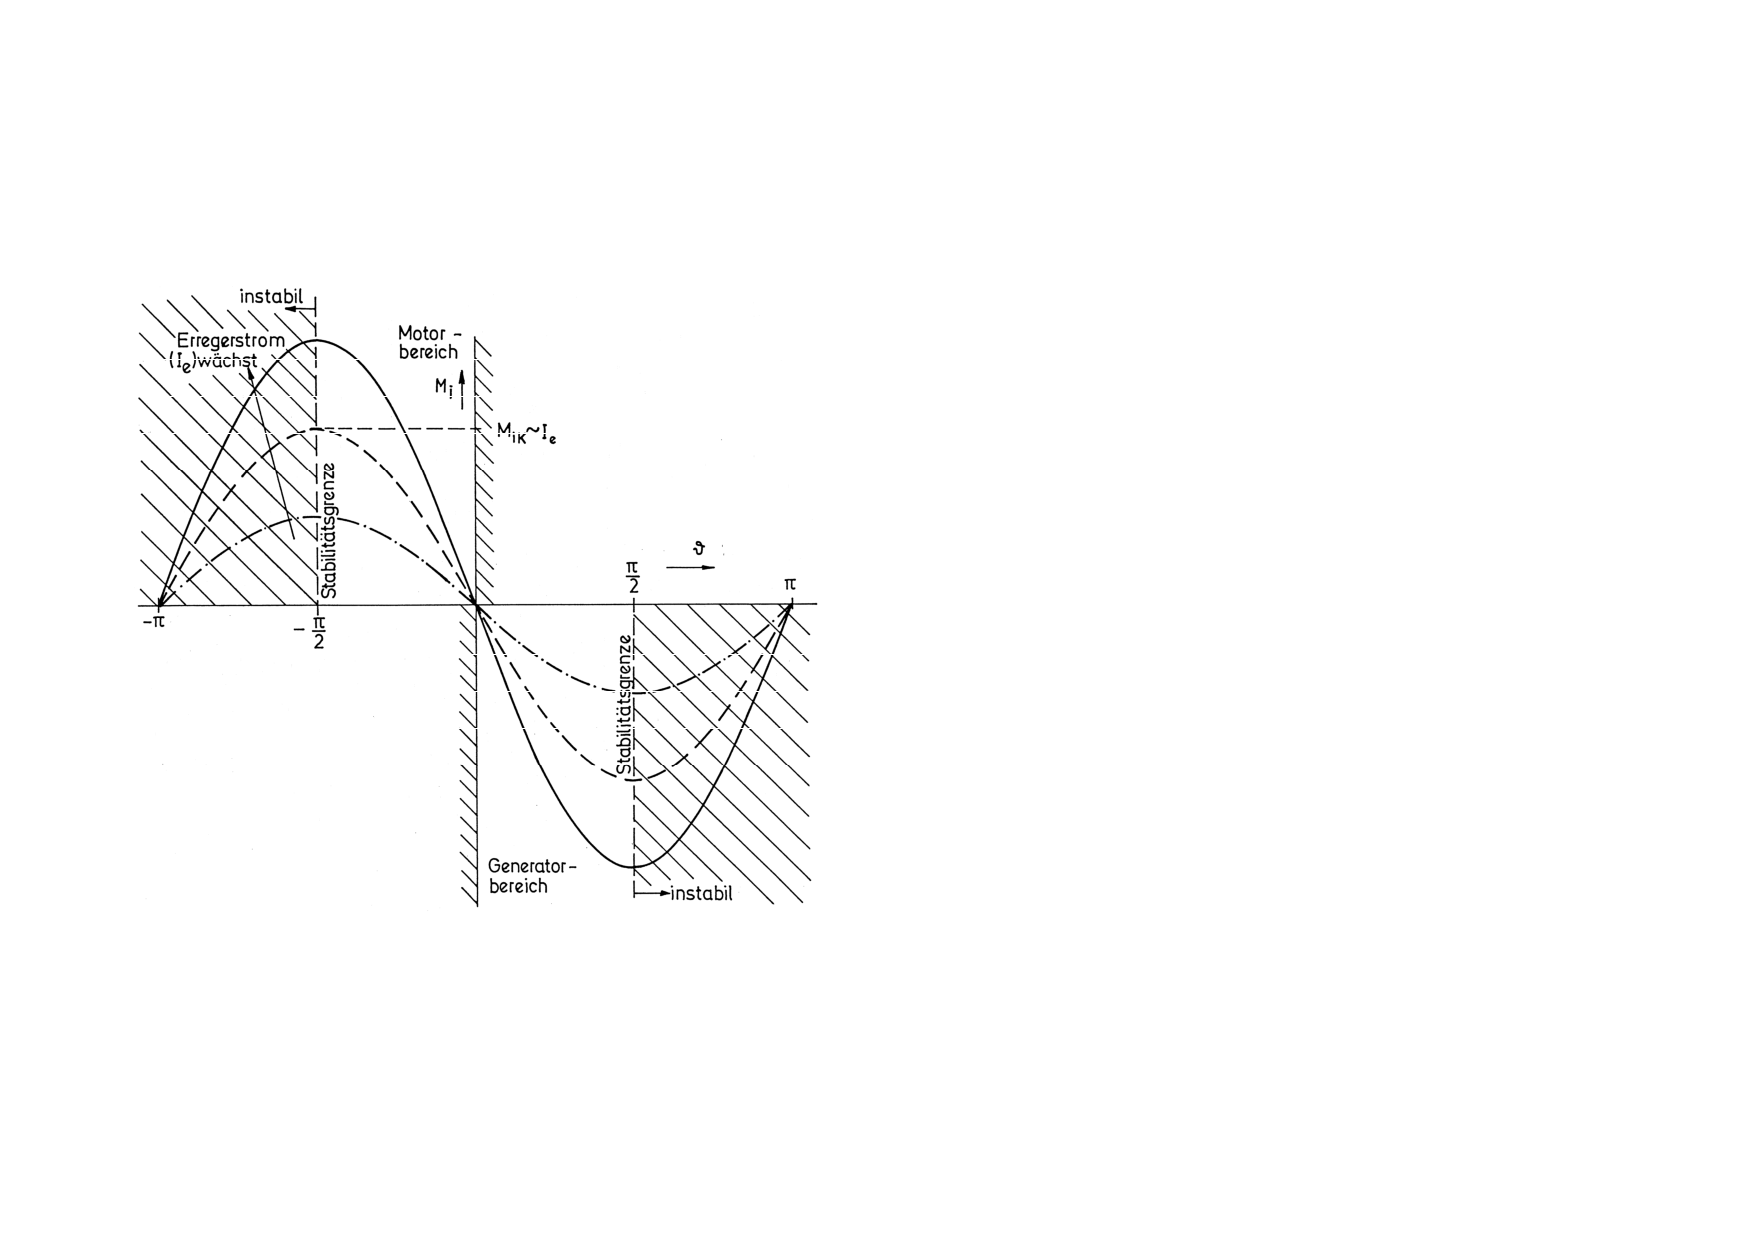
\includegraphics[width=0.5\textwidth]{img/SM_Kennlinie.pdf}
\end{figure}
\subsection*{Formeln}
\fancyformula{Verhältnis mechanischer Polradwinkel zu elektrischem Polradwinkel:}{
	\[
		\alpha_p = \dfrac{\theta}{p}
	\]
}

\fancyformula{Verhältnis von $I_{1W}$ zum elektrischen Polradwinkel}{
	\[
		I_{1W}=I_1 \cdot cos(\phi)=\dfrac{U_p}{\omega L_1}sin(-\theta)=\dfrac{U_{1N}}{\omega L_1}\dfrac{I_e}{I_{e0}}sin(-\theta)
	\]
}

\fancyformula{Drehmoment in Abhängigkeit von Polradwinkel}{
	\[
		M_i=M_{iK}sin(-\theta)=3\dfrac{p}{\omega^2L_1}U_1U_{1N}\dfrac{I_e}{I_{e0}}sin(-\theta)
	\]
	\begin{center}
	Wobei: $M_{iK}=3\dfrac{p}{\omega^2L_1}U_1U_{1N}\dfrac{I_e}{I_{e0}}$
	\end{center}
}

\fancyformula{Proportionalitäten}{
	\[
		\frac{M_i}{M_{iN}} = \frac{I_{1W}}{I_{1WN}} = \frac{P_i}{P_{iN}}
	\]
}

\newpage
\section*{Transformator}
\fancythumb{Trafo}{olive}
%TODO: Festgekoppelter Transformator, mehr Schaltgruppen-Übertragungsverhältnisse

\subsection*{Schaltgruppen}
Typische Verschaltungen von Drehstromtransformatoren sind: Dreieckschaltung ($\triangle$, D), Sternschaltung ($\Yup$, Y) und Zickzackschaltung (Z).
\vspace{.5em}

Die Schaltgruppenbezeichnung besteht aus
\begin{tabular}{r p{11cm}}
	\textbf{1. Kennbuchstabe} & Schaltung der Oberspannungsseite (Y, D, Z) \\
	\textbf{2. Kennbuchstabe} & Schaltung der Unterspannungsseite (y, d, z) \\
	\textbf{3. Kennzahl $n$} & Stundenzahl, die Zeiger der Unterspannungsseite eilen denen der Oberspannungsseite um $n \cdot 30^\circ$ nach
\end{tabular}

\subsubsection*{Übertragungsverhältnis nach Schaltgruppe}
\begin{tabular}{c c c c}
	$\ddot u = \frac{w_1}{w_2}$ & $\ddot u = \frac{w_1}{\sqrt{3} ~ w_2}$ & $\ddot u = \frac{\sqrt{3} ~ w_1}{w_2}$ & $\ddot u = \frac{2 ~ w_1}{\sqrt{3} ~ w_2}$ \\ \hline \rule{0pt}{3ex}
	Yy0 & Dy5 & Yd5 & Yz5 \\
	Dd0 & Dy11 & Yd11
\end{tabular}

\subsection*{Ersatzschaltbilder}
\subsubsection*{Vollständiges Ersatzschaltbild ohne idealen Transformator}
\begin{figure}[h]\centering
	\begin{circuitikz}[european, scale=1, font=\large]
	\draw
		(0,3)
		to [short, i=$\underline{I}_1$, o-](1.0,3)
		to [R=$R_1$](3, 3)
		to [L=$L_{\sigma1}$](6,3)
		to [L=$L_{h1}$, i>^=$\underline{I}_{m1}$, *-*] (6,0)
		(6.0,3.0)
		to [L=$L_{\sigma2}'$](8.9,3)
		to [short, i>^=$\underline{I}_1^i$](9.1,3)
		to [R=$R_{2}'$, -o](12.0,3)
		to [short, i<^=$\underline{I}_2'$](14,3)
		to [R, l=$\underline Z_V'$](14,0)
		to [short, -o](12,0)
		to [short, -o](0,0);

	\draw[->, >=latex] (0,2.8) -- (0,0.2) node [pos=0.5, left] {$\underline U_1$};
	\draw[->, >=latex] (12,2.8) -- (12,0.2) node [pos=0.5, left] {$\underline U_2'$};
	\draw[->, >=latex] (5.5,2.5) -- (5.5,0.5) node [pos=0.5, left] {$\underline U_{h1} = \underline U_{h2}'$};
	\end{circuitikz}
	\caption*{Gestrichene ($'$) Größen sind auf die Primärseite bezogen}
\end{figure}

\subsubsection*{Vereinfachtes Ersatzschaltbild 1. Art}
Näherung $|\underline I_{m1}| \ll |\underline I_1^i|$ ergibt mit $R_k = R_1 + R_2' \quad \mathrm{und} \quad L_k = L_{\sigma1} + L_{\sigma2}'$
\begin{figure}[h]\centering
	\begin{circuitikz}[european, scale=1, font=\large]
	\draw
		(0,3)
		to [short, i=$\underline{I}_1$, o-](1.0,3)
		to [L=$L_{h1}$, i>^=$\underline{I}_{m1}$, *-*] (1,0)
		(1.0,3.0)
		to [R=$R_k$](4,3)
		to [L=$L_k$, -o](7,3)
		to [short, i<^=$\underline{I}_2'$](9,3)
		to [R, l=$\underline Z_V'$] (9,0)
		to [short, -o](7,0)
		to [short, -o]	(0,0);

	\draw[->, >=latex] (0,2.8) -- (0,0.2) node [pos=0.5, left] {$\underline U_1$};
	\draw[->, >=latex] (7,2.8) -- (7,0.2) node [pos=0.5, left] {$\underline U_2'$};
	\end{circuitikz}
\end{figure}

\subsubsection*{Vereinfachtes Ersatzschaltbild 2. Art}
Näherung $|\underline I_{m1}| \approx 0$ ergibt:
\begin{figure}[H]\centering
	\begin{circuitikz}[european, scale=1, font=\large]
	\draw
		(0,3)
		to [short, i=$\underline{I}_1$, o-](1.0,3)
		to [R, l=$\underline Z_k \textnormal{=} R_k + j \omega L_k$, -o](4,3)
		to [short](5,3)
		to [R, l=$\underline Z_V'$] (5,0)
		to [short, -o](4,0)
		to [short, -o](0,0);

	\draw[->, >=latex] (0,2.8) -- (0,0.2) node [pos=0.5, left] {$\underline U_1$};
	\draw[->, >=latex] (4,2.8) -- (4,0.2) node [pos=0.5, left] {$\underline U_2'$};
	\end{circuitikz}
\end{figure}

\subsection*{Leistungsbilanz}
\begin{figure}[h]
	\centering
	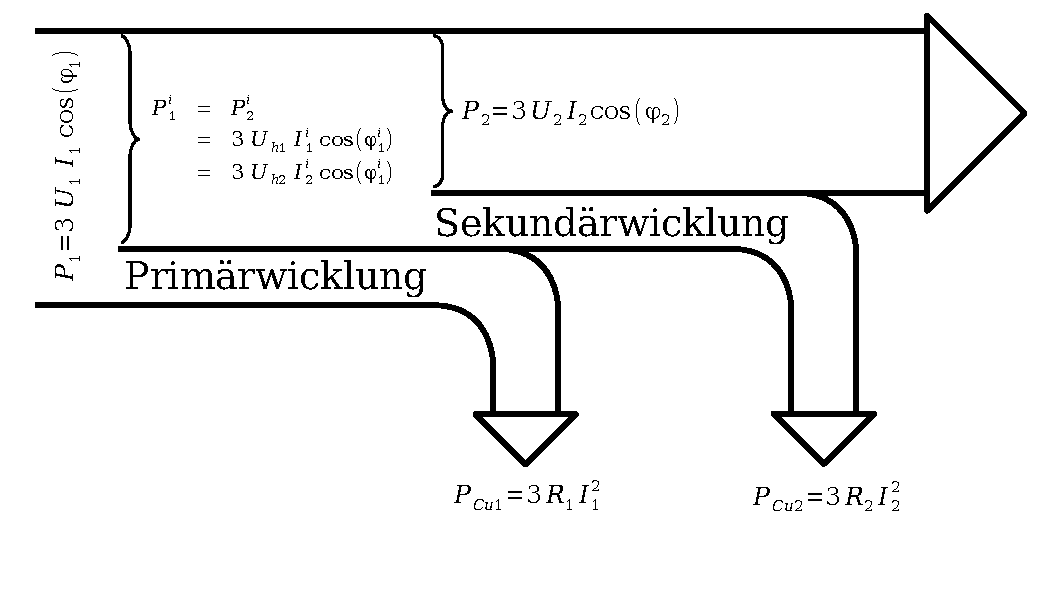
\includegraphics[width=0.8\textwidth]{img/transformator_leistungsbilanz.pdf}
	\caption*{Faktor $3$ ist spezifisch für dreiphasigen Drehstromtransformator}
\end{figure}

\subsection*{Impedanzwandlung}
Das Übertragunsverhältnis $\ddot u$ wird (meist) so angegeben, dass $\ddot u > 1$. Für $\underline Z_{HV}$ auf der Hochspannungsseite und $\underline Z_{LV}$ auf der Niederspannungsseite gilt:
\[
	\underline Z_{HV} = \ddot u^2 ~ \underline Z_{LV}
\]
\textbf{Die auf die Hochspannungsebene bezogene Impedanz ist größer!}

\subsection*{Kenngrößen}
\subsubsection*{Kurzschlussspannung}
Die \textit{Nennkurzschlussspannung} $\underline U_{1k}$ ist die Sternspannung, die an den Primärklemmen anliegt, wenn bei kurzgeschlossenen Sekundärklemmen an den Primärklemmen reeller Nennstrom fließt, d.h. $\arg(\underline I) = 0$. Wird $U_{1k}$ bzw. $u_{1k}$ rein betragsmäßig angegeben, so handelt es sich um den positiven Imaginärteil des Wertes ($\rightarrow$ Kurzschlussimpedanz ist reine Reaktanz).

\vspace{.5em}
Häufig wird die auf die Nennspannung bezogene \textit{relative Nennkurzschlussspannung} $\underline u_{kN}$ angegeben mit:
\[
	\underline u_{kN} = \frac{\underline U_{1kN}}{U_{1N}} = \frac{\sqrt{3} ~ \underline U_{1k\Yup}}{U_{1N}}
\]

\subsubsection*{Kurzschlussimpedanz}
Die \textit{Kurzschlussimpedanz} $\underline Z_k$ entspricht der Impedanz im vereinfachten ESB 2. Art. Es gilt:
\[
	\underline Z_k = \underline u_{kN} ~ \frac{U_N^2}{S_N} \textnormal{, wobei $\underline Z_k$ bezogen auf Seite mit Spannung $U_N$}
\]

\raggedright
\vspace{12pt}
\footnotesize
\begin{tabular}{r p{13cm}}
	\sffamily\textbf{Indizes:} & \rmfamily \textbf{1} = Primärseite, \textbf{2} = Sekundärseite, \textbf{N} = Nennwert (insbes. $\triangle$-Schaltung), \textbf{k} = sekundärseitiger Kurzschluss
\end{tabular}
\normalsize

\subsection*{Parallelbetrieb}
Parallelbetrieb ist erlaubt wenn
\begin{itemize}
\item Gleiches Übersetzungsverhältnis
\item Gleiche Stundenzahl der Schaltgruppe
\item Keiner der Transformatoren wird außerhalb des zulässigen Betriebsbereichs betrieben (die Ströme teilen sich nach dem ESB 2. Art gemäß den Kurzschlussimpedanzen auf \mbox{$\rightarrow$ Stromteiler}).
\end{itemize}
Die Belastung der Transformatoren erfolgt automatisch proportional zu den Nennleistungenen, wenn beide die gleichen (relativen) Kurzschlussspannungen aufweisen.

\newpage
\section*{Drehstromverbraucher}
\fancythumb{\huge $\Yup ~ \mathrm{/} ~ \triangle$}{darkgray}

\newpage
\section*{Anhang}
\fancythumb{Anhang}{black}
\subsection{Herleitung Schlupfgerade Asynchronmaschine} \label{ssec:appendix_asm_slip}
\begin{figure}[h]
	\centering
	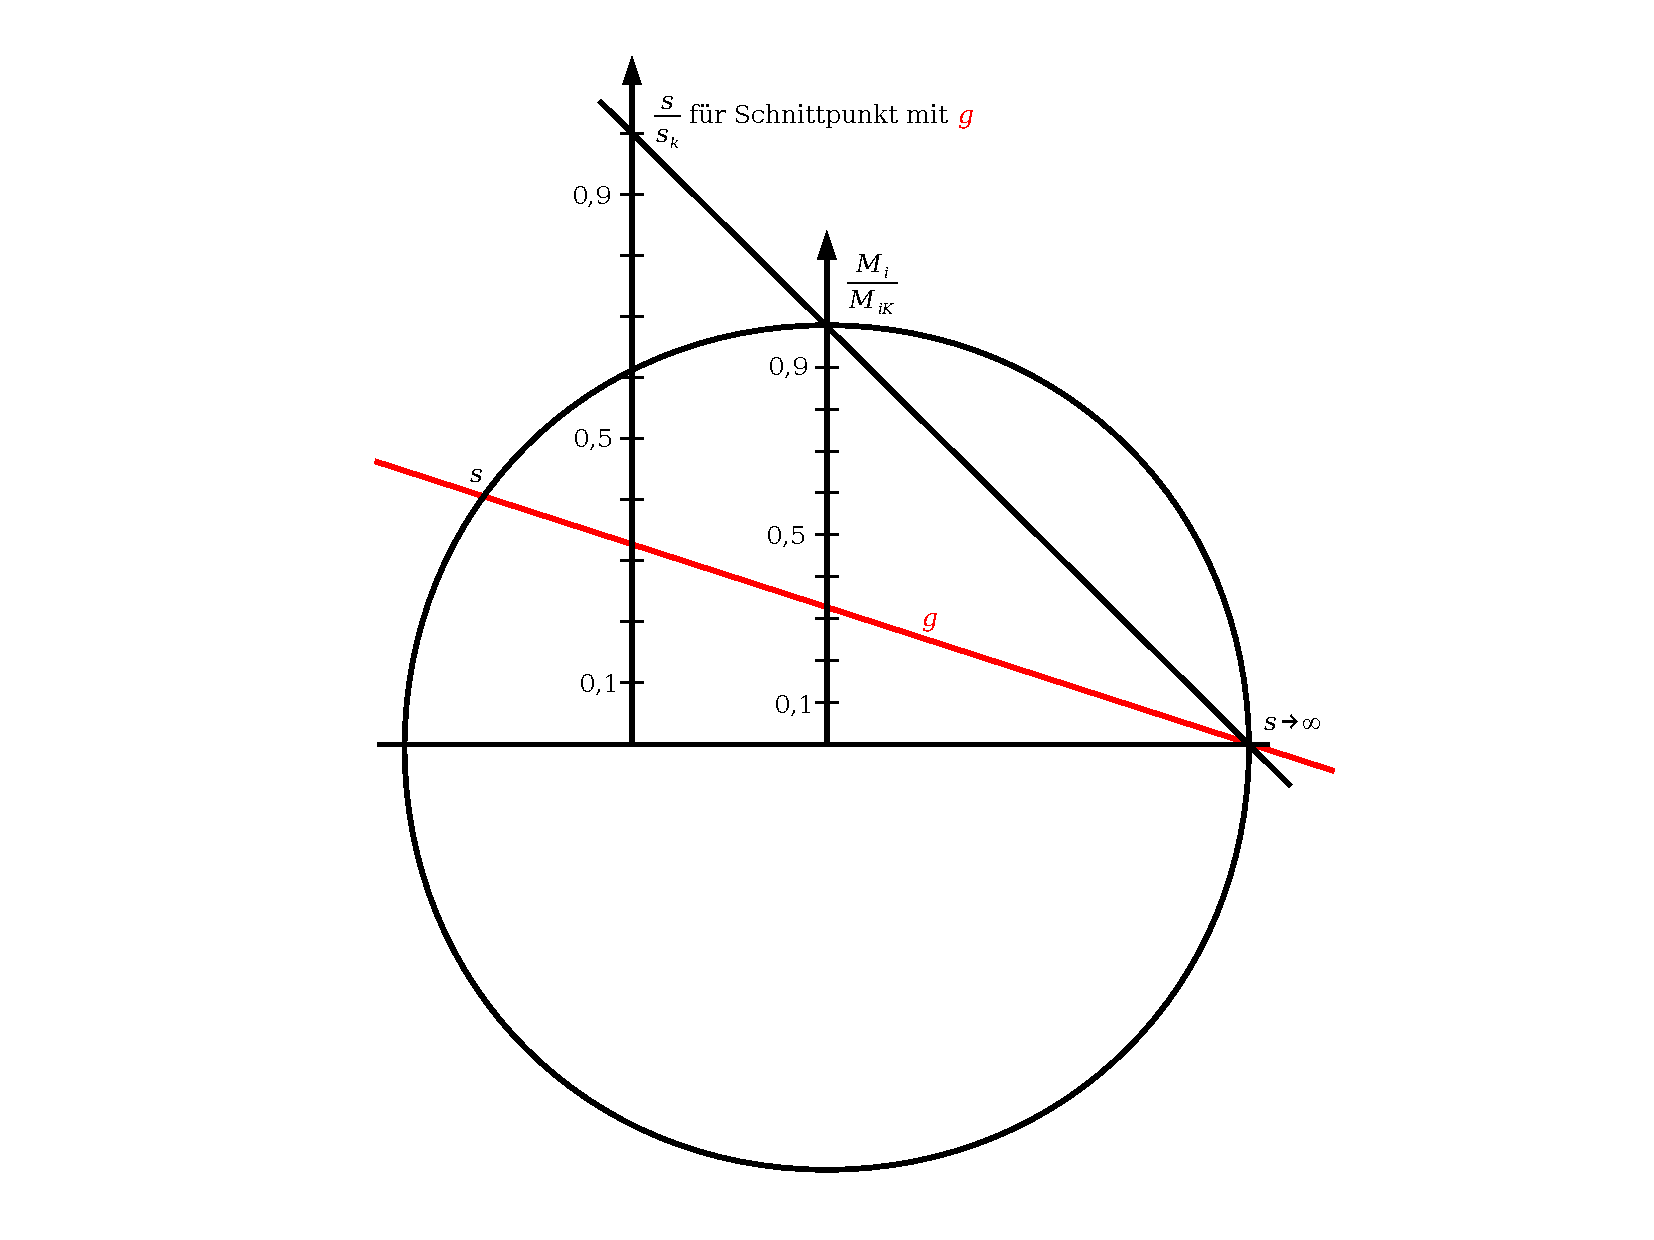
\includegraphics[width=0.8\textwidth]{img/asynchronmaschine_schlupfgerade_verschoben.pdf}
	\caption*{Heylandkreis - Der Schlupf an Stelle $s$ soll bestimmt werden}
\end{figure}

\paragraph{Problem:} Wir möchten den Wert des Schlupfes für einen beliebigen Punkt auf dem Heylandkreis (die Ortskurve des Statorstroms in der komplexen Ebene) bestimmen. Der Schlupf hat allerdings keinen linearen Zusammenhang mit dem Mittelpunktswinkel. Der Kippschlupf sei bekannt.

\paragraph{Behauptung:} Durch Konstruktion einer Skala $s \over s_k$ wie in der obigen Grafik, sodass der Wert $1,0$ der Skala durch die Gerade vom Punkt $s \to \infty$ durch den Punkt des Kippschlupfes ("oben" im Kreis) gegeben ist, lässt sich der Schlupf eines beliebigen Punktes $s$ auf dem Heylandkreis ablesen. Dazu wird eine Gerade $g$ durch den Punkt $s \to \infty$ und $s$ konstruiert. Der Wert $s \over s_k$ kann nun am Schnittpunkt dieser Gerade mit der Skala abgelesen werden.

\paragraph{Beweis: } Zeige die Behauptung erst für den Fall, dass sich die $s \over s_k$-Skala im horizontalen Mittelpunkt des Kreises befindet und verallgemeinere dann. Der Kreis habe den Radius $1$, da der Zusammenhang $\frac{M_i}{M_{iN}} = \frac{I_{1W}}{I_{1WN}}$ gilt (d.h. Normierung des Stroms auf ein Drehmoment ist erlaubt, ohne die Grafik zu verzerren) und da hier auf das Kippdrehmoment $M_{iK}$ normiert wurde. Für diese Herleitung liege der abzulesende Punkt in der linken Halbebene des Kreises.

\begin{figure}[H]
	\centering
	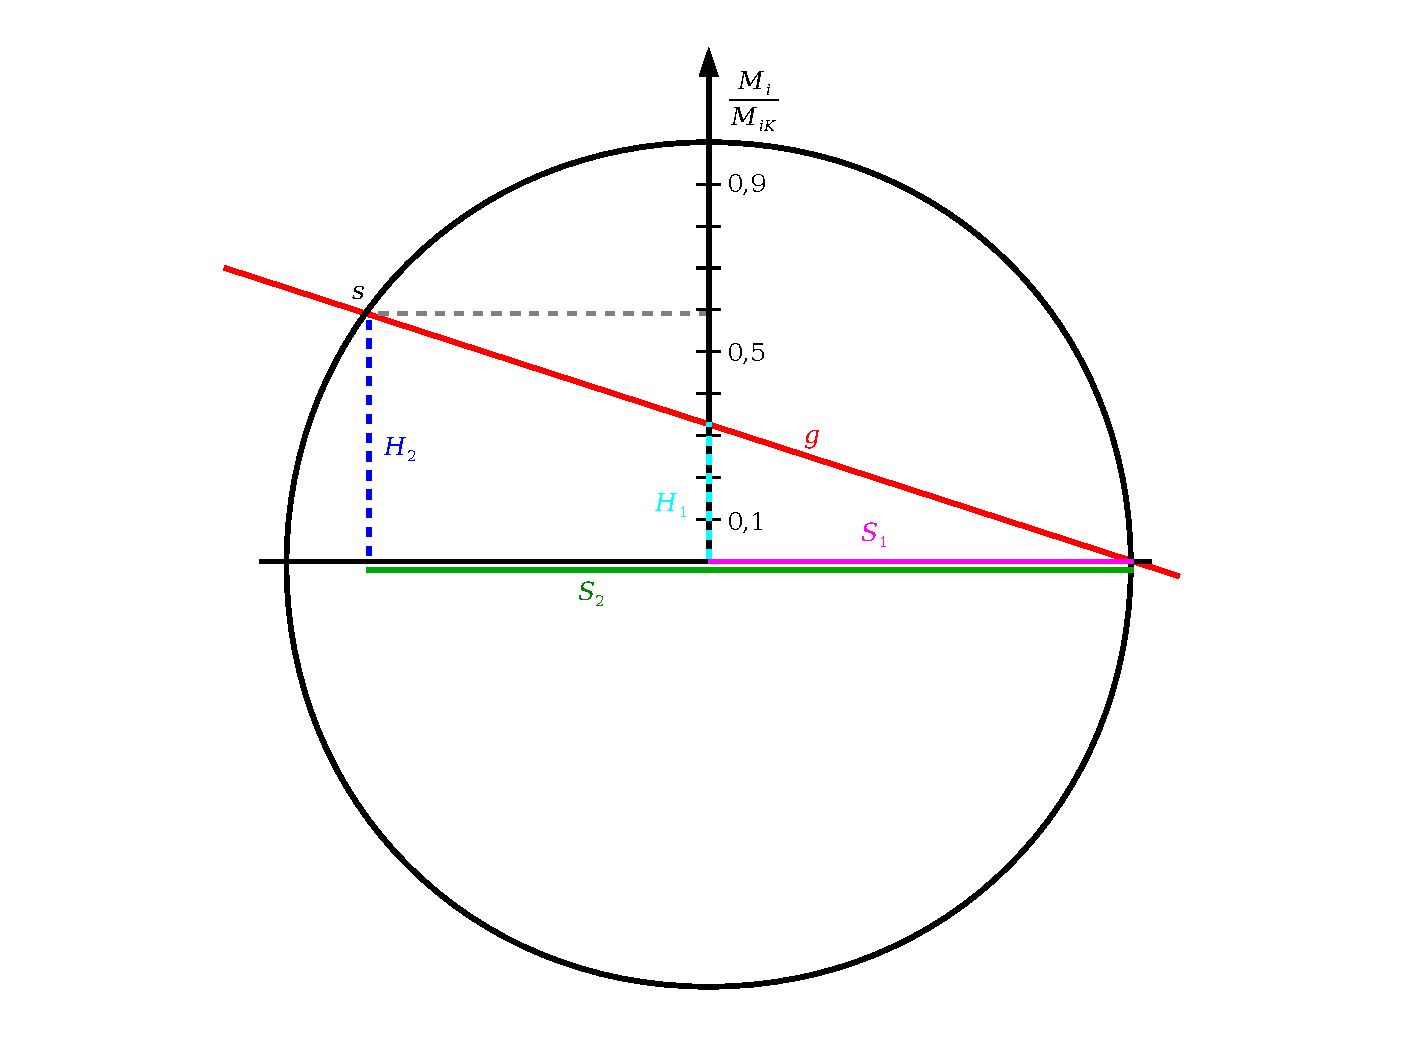
\includegraphics[width=0.8\textwidth]{img/asynchronmaschine_schlupfgerade.pdf}
	\caption*{Schlupfgerade mit Strecken für Strahlensatz}
\end{figure}

Der 2. Strahlensatz lässt mit den Bezeichnungen der Grafik formulieren:
\[
	\frac{H_1}{H_2} = \frac{S_1}{S_2} \implies H_1 = H_2 ~ \frac{S_1}{S_2}
\]

Sei nun das innere Drehmoment des abzulesenden Punktes $M_i$ sowie $M_{ik}$ bekannt. So gilt sofort mit der Normierung auf $M_{iK}$ (Kreisradius 1):
\[
	H_2 = \frac{M_i}{M_{iK}} \quad \mathrm{und} \quad S_1 = 1
\]

$S_2$ kann außerdem einfach aus dem bekannten $H_2$ und dem bekannten Kreisradius 1 berechnet werden:
\[
	H_2^2 + (S_2 - S_1)^2 = 1 \implies S_2 = \sqrt{1 - H_2^2} + S_1 = \sqrt{1 - \left( \frac{M_i}{M_{iK}} \right)^2} + 1
\]

Somit ergibt sich für $H_1$ durch einsetzen in den Strahlensatz:
\[
	H_1 = \frac{\frac{M_i}{M_{iK}}}{\sqrt{1 - \left( \frac{M_i}{M_{iK}} \right)^2} + 1}
\]

Die Behauptung ist nun, dass $H_1 \overset{!}{=} \frac{s}{s_k}$. Dies ist gezeigt, wenn $H_1$ die Kloss'sche Formel erfüllt, d.h.:
\[
	\frac{M_i}{M_{iK}} = \frac{2}{\frac{s}{s_K} + \frac{s_K}{s}} \overset{!}{=} \frac{2}{H_1 + \frac{1}{H_1}}
\]

Berechne $H_1 + \frac{1}{H_1}$:
\begin{align*}
H_1 + \frac{1}{H_1}
		&= \frac{\frac{M_i}{M_{iK}}}{\sqrt{1 - \left( \frac{M_i}{M_{iK}} \right)^2} + 1} + \frac{\sqrt{1 - \left( \frac{M_i}{M_{iK}} \right)^2} + 1}{\frac{M_i}{M_{iK}}} \\
		&= \frac{M_i}{\sqrt{M_{iK}^2 - M_i^2} + M_{iK}} + \frac{\sqrt{M_{iK}^2 - M_i^2} + M_{iK}}{M_i} = \frac{M_i^2 + \left(\sqrt{M_{iK}^2 - M_i^2} + M_{iK}\right)^2}{\left(\sqrt{M_{iK}^2 - M_i^2} + M_{iK}\right)~M_i} \\
		&= \frac{M_i^2 + M_{iK}^2 - M_i^2 + M_{iK}^2 + 2 ~ M_{iK} ~ \sqrt{M_{iK}^2 - M_i^2}}{\left(\sqrt{M_{iK}^2 - M_i^2} + M_{iK}\right)~M_i} \\
		&= \frac{2 ~ M_{iK}^2 + 2 ~ M_{iK} ~ \sqrt{M_{iK}^2 - M_i^2}}{\left(\sqrt{M_{iK}^2 - M_i^2} + M_{iK}\right)~M_i} = \frac{2 \; M_{iK}}{M_i} ~ \frac{M_{iK} + \sqrt{M_{iK}^2 - M_i^2}}{\sqrt{M_{iK}^2 - M_i^2} + M_{iK}} = 2 ~ \frac{M_{iK}}{M_i}
\end{align*}

Einsetzen in die Kloss'sche Formel ergibt:
\[
	\frac{M_i}{M_{iK}} \overset{!}{=} \frac{2}{2 ~ \frac{M_{iK}}{M_i}} \Leftrightarrow 1 = 1
\]

Das heißt, der auf der vertikalen Gerade durch den Kreismittelpunkt abgelesene, normierte Wert ist tatsächlich das gesuchte $s \over s_k$-Verhältnis. Ein Verschieben der Gerade ändert bei entsprechender Anpassung der Skala den abgelesenen Wert nicht ($\rightarrow$ Strahlensatz), somit gilt auch die anfängliche Behauptung. Der Beweis für Punkte auf dem Kreis in anderen Quadranten erfolgt analog. $\square$

\end{document}